À présent que la stabilité des deux méthodes ImEx ont été comparées au \textit{splitting} d'opérateur, 
il est naturel de poursuivre par une expérience numérique pour qualifier la convergence de chaque méthode et 
d'évaluer la pertinence des méthodes ImEx face au \textit{splitting}.
\subsubsection{Expérience sur l'équation de Nagumo}
    \paragraph{Présentation de l'expérience}
    L'expérience est réalisée sur l'équation de Nagumo 1D à partir d'une solution initiale correspondant au profil de l'onde propagative de l'équation (voir \ref{par:analyser_operateurs_nagumo}).
    Succinctement, la simulation à lieu sur le domaine spatial $[-20,+20]$ entre $t=0$ et $t=3$.
    La grille spatial est divisée en $2^{13}$ cellules ce qui équivaut à un pas d'espace $\Delta t \approx 4.8 \, 10^{-3}$.
    Des conditions de Neumann homogènes et une vitesse de propagation adaptées permettent de maintenir le front d'onde au centre du domaine et 
    de négliger les effets de bords afin de comparer à la solution analytique exacte d'onde propagative. Les erreurs sont calculés sur le domaine $[-5,+5]$ pour ce centrer sur l'étude du front d'onde.
    \paragraph{Résultats}
    Les résultats de l'expérience sont présentés en \ref{fig:imex_vs_splitting},
    \begin{figure}[ht]
        \centering
        \begin{subfigure}{\textwidth}
            \centering
            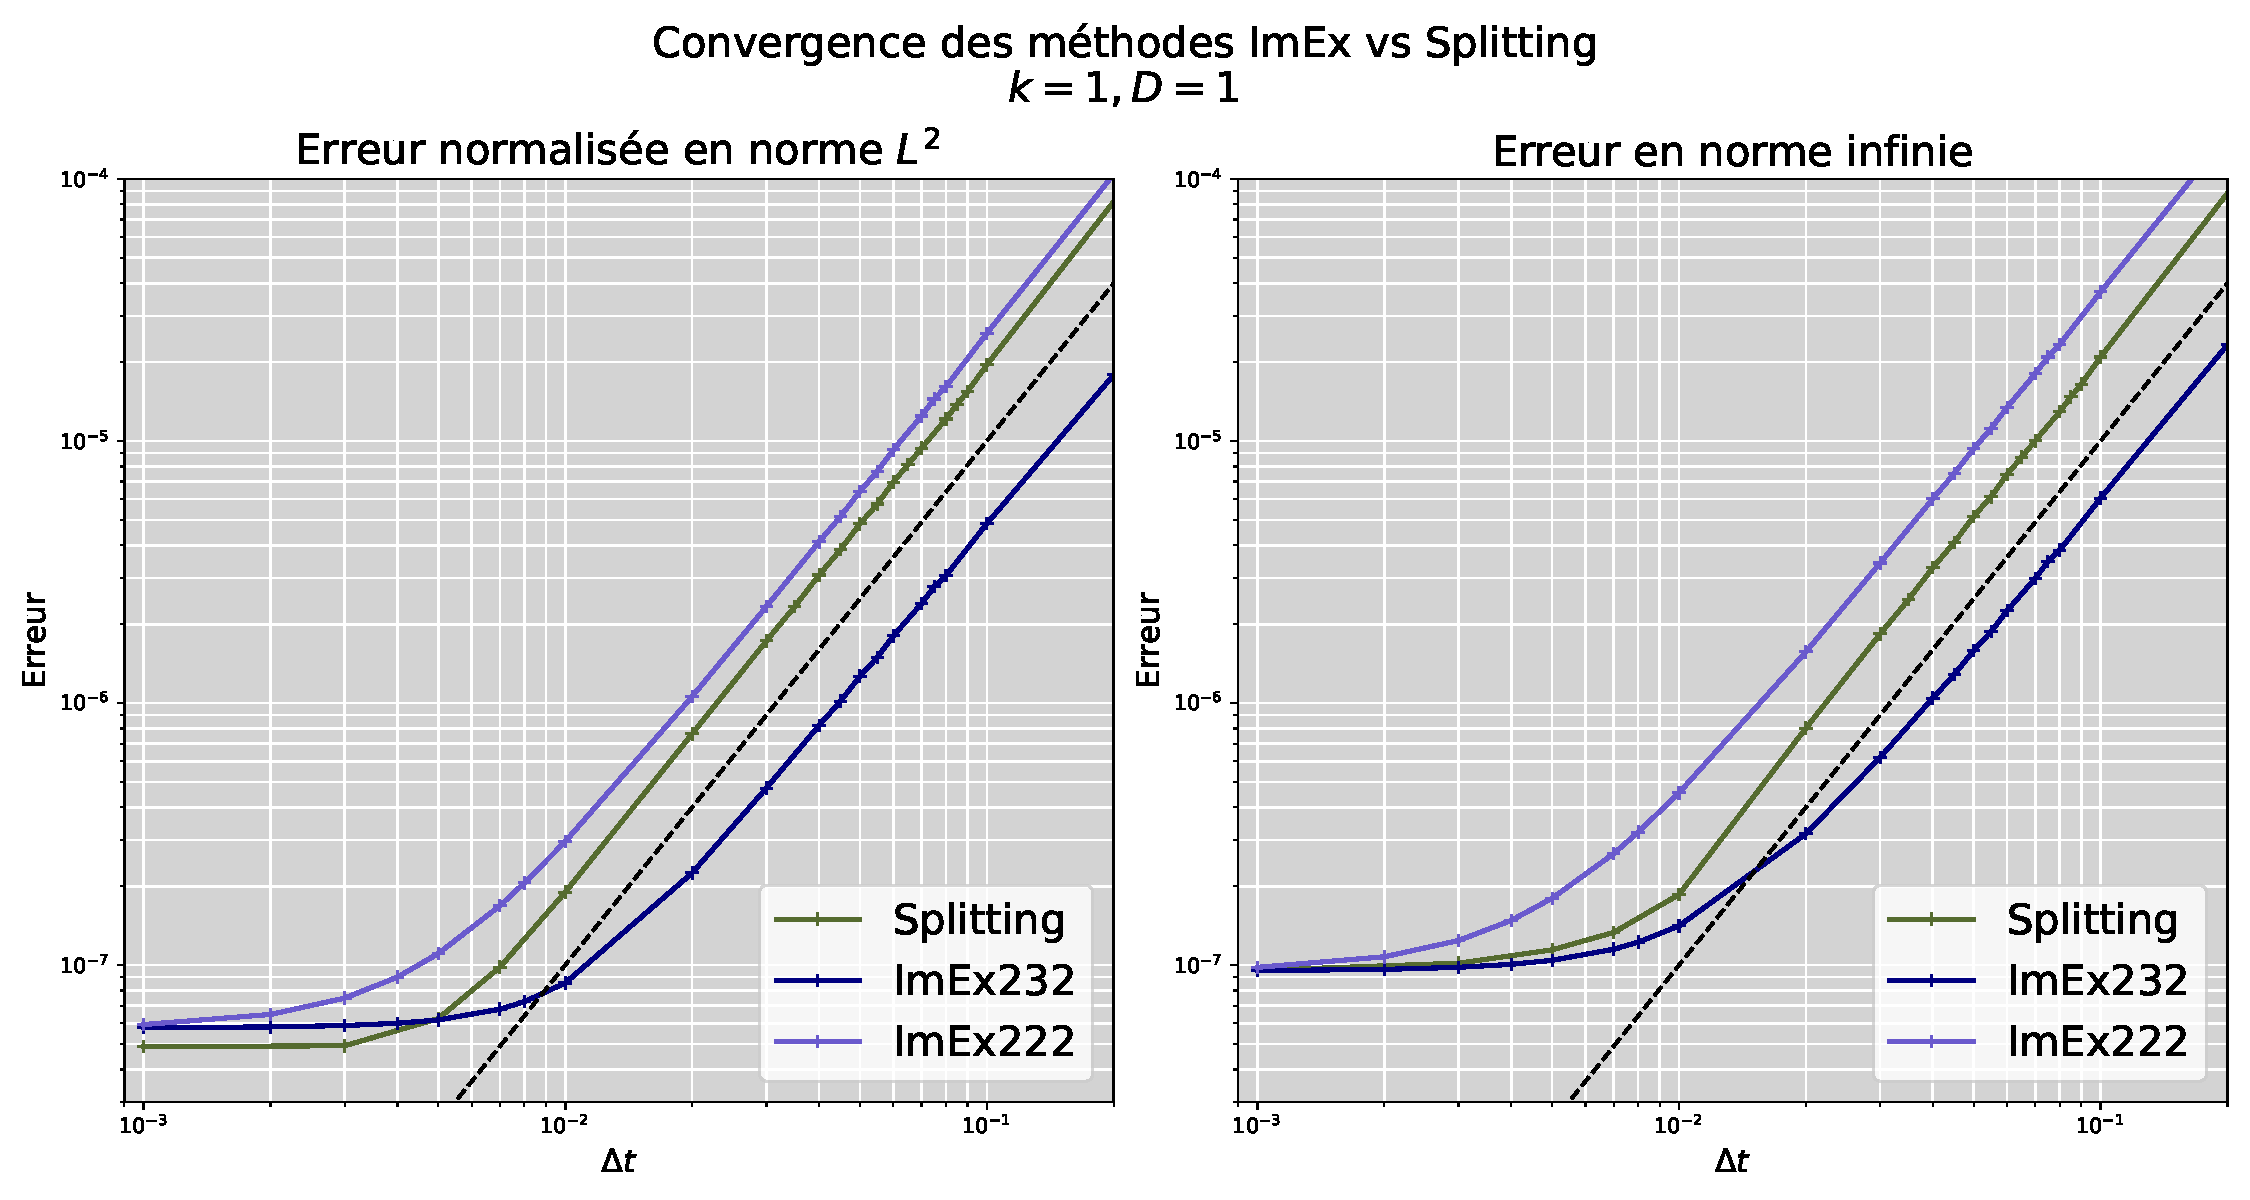
\includegraphics[width=\linewidth]{media/4_travail/2_nagumo/convergence/ImEx_vs_splitting_k1_D1.pdf}
            \caption{} % légende à compléter
            \label{fig:imex_k1_d1}
        \end{subfigure}
    \begin{subfigure}{\textwidth}
        \centering
        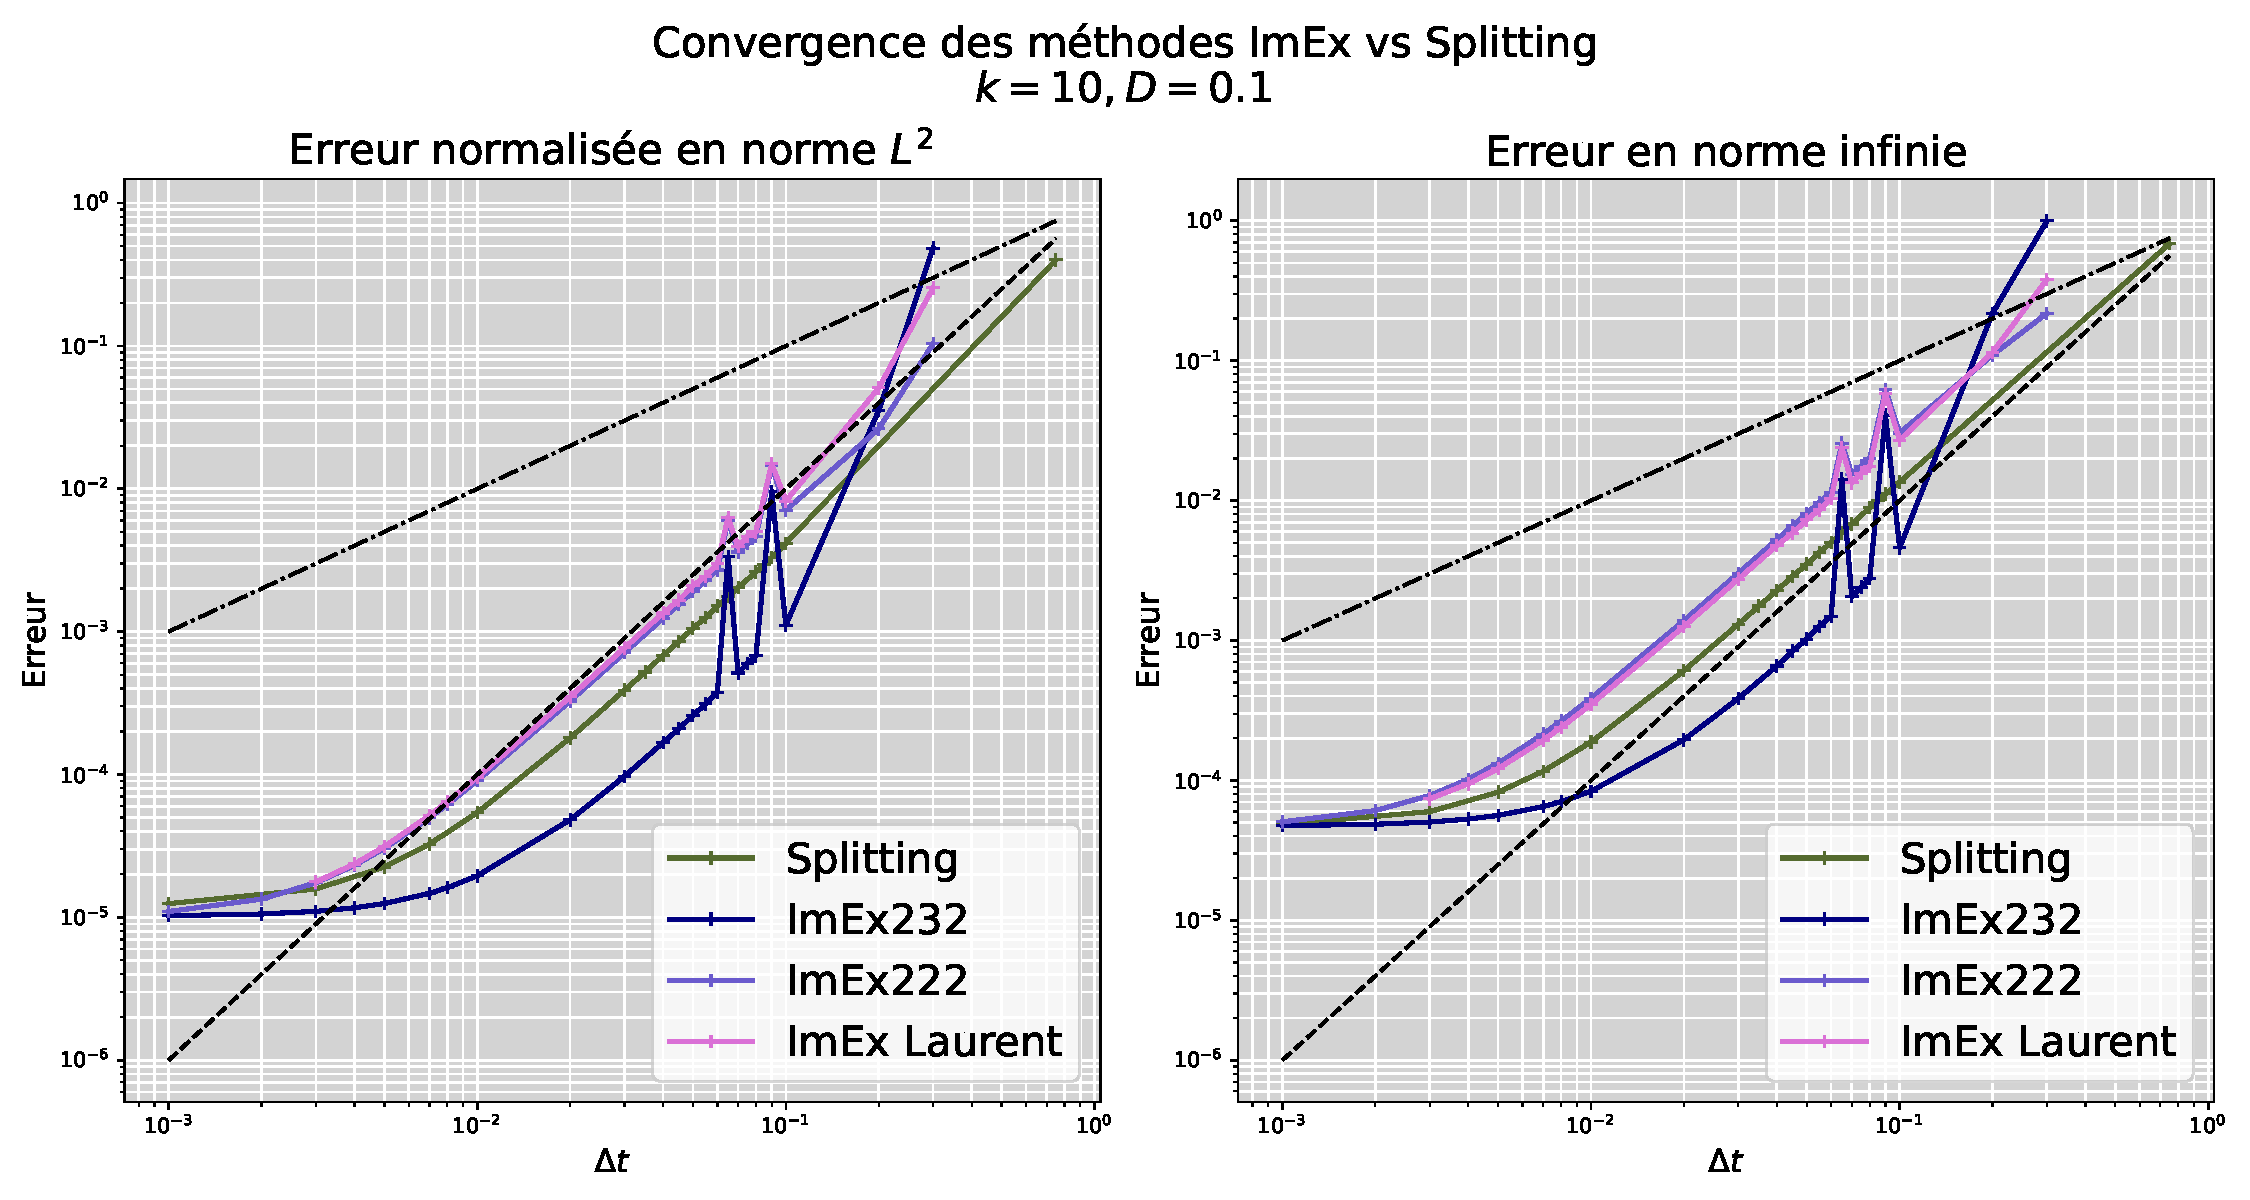
\includegraphics[width=\linewidth]{media/4_travail/2_nagumo/convergence/ImEx_vs_splitting_k10_D0.1.pdf}
        \caption{} % légende à compléter
        \label{fig:imex_k10_d01}
    \end{subfigure}
    \caption{} % légende globale de la figure
    \label{fig:imex_vs_splitting}
    \end{figure}
    \paragraph{Conclusion}
\subsubsection{Expérience sur l'équation de Nagumo - Complément avec AMR}